\documentclass[conference]{IEEEtran}
\IEEEoverridecommandlockouts
\usepackage{cite}
\usepackage{amsmath,amssymb,amsfonts}
\usepackage{algorithm}
\usepackage{algpseudocode}
\usepackage{graphicx}
\usepackage{textcomp}
\usepackage[table]{xcolor}
\usepackage{booktabs}
\usepackage{multirow}
\def\BibTeX{{\rm B\kern-.05em{\sc i\kern-.025em b}\kern-.08em
    T\kern-.1667em\lower.7ex\hbox{E}\kern-.125emX}}

\begin{document}

\title{Revisiting DropGaussian: An Empirical Study of\\
Opacity-Aware Dropout and Drop-Aware Densification\\
for Sparse-View Gaussian Splatting}

\author{\IEEEauthorblockN{Student Name}
\IEEEauthorblockA{SLAM Technology --- Final Project\\
Student ID}}

\maketitle

\begin{abstract}
DropGaussian is a recent structural regularizer for sparse-view 3D Gaussian
Splatting (3DGS) that randomly eliminates Gaussians during training so that the
remaining ones receive larger gradients, alleviating overfitting under sparse
inputs. We first reproduce DropGaussian on the LLFF 3-view benchmark, matching
the reported 8-scene mean within 1.6\% PSNR. We then identify two independent
methodological weaknesses: (i) the dropout is \emph{uniform}, treating all
Gaussians as equally important despite their highly skewed opacity distribution,
and (ii) the densification statistics are computed from the \emph{dropout-perturbed}
gradients, silently coupling the regularizer with the cloning/splitting heuristic.
We turn each into a falsifiable hypothesis and implement two improvements: an
opacity-aware adaptive dropout with unbiased, variance-bounded compensation (H1)
and a drop-aware densification gradient correction (H2). Through a noise-controlled
8-scene ablation we find that H1 does \emph{not} hold---protecting high-opacity
Gaussians weakens the very ``break-the-dominance'' mechanism that makes DropGaussian
work---while H2 yields a small but consistent quality gain (+0.22\,dB, 6/8 scenes)
and, more convincingly, a \emph{deterministic} $\sim$10\% reduction in the number of
Gaussians on all eight scenes at equal-or-better SSIM/LPIPS and negligible cost. We
quantify the run-to-run noise floor of the non-deterministic CUDA rasterizer, show
that the compactness result is noise-free, and discuss why dropout-level refinements
have diminishing returns on this already-strong baseline. We report all outcomes,
positive and negative, honestly.
\end{abstract}

\begin{IEEEkeywords}
3D Gaussian Splatting, sparse-view synthesis, dropout, structural regularization,
densification, novel view synthesis
\end{IEEEkeywords}

\section{Introduction}
3D Gaussian Splatting (3DGS)~\cite{kerbl3Dgaussians} represents a scene as a set of
anisotropic 3D Gaussians, each with a position, covariance, opacity and view-dependent
color, and renders them by differentiable rasterization. It attains real-time,
photorealistic novel view synthesis and has rapidly become a default explicit
radiance-field representation. Its quality, however, hinges on \emph{dense} multi-view
supervision. When only a handful of input views are available---the sparse-view
regime relevant to casual capture and robotics/SLAM front-ends---3DGS overfits the
training views: redundant Gaussians proliferate, opacities drift, and the held-out
views exhibit floaters, holes and broken geometry.

A growing body of work tackles sparse-view 3DGS by injecting external knowledge
(monocular-depth priors, cross-field co-regularization, generative priors).
DropGaussian~\cite{park2025dropgaussian} stands out by being \emph{prior-free}: it
borrows the idea of Dropout from deep networks and randomly \emph{eliminates}
Gaussians during the forward pass. Concretely, at iteration $t$ it draws a dropout
rate $p_t=0.2\,(t/T)$ that grows linearly with training, multiplies each Gaussian's
opacity by an i.i.d.\ inverted-dropout mask, and rescales survivors by $1/(1-p_t)$.
The intuition is that removing a random subset forces the remaining Gaussians to
``stand in'' for the missing ones, distributing gradients more evenly and preventing
a few dominant Gaussians from memorizing the training views. Despite its simplicity,
DropGaussian is competitive with prior-based methods.

Precisely because the idea is simple and prior-free, it is a clean object of study:
every design choice is exposed and can be questioned. Following the
\emph{read $\rightarrow$ find flaws $\rightarrow$ hypothesize $\rightarrow$ implement
$\rightarrow$ experiment} loop, this work makes two contributions:
\begin{itemize}
\item We \textbf{reproduce} DropGaussian on the eight LLFF 3-view scenes and confirm
its reported gains over vanilla 3DGS, establishing a faithful, noise-characterized
baseline (Sec.~\ref{sec:baseline}).
\item We \textbf{analyze} two \emph{independent} weaknesses---the uniformity of the
dropout (L1) and its pollution of the densification statistics (L2)---turn each into
a falsifiable hypothesis, implement both (H1, H2), and evaluate them with a
noise-controlled 8-scene ablation (Sec.~\ref{sec:limitations}--\ref{sec:exp}). We
report a negative result (H1) and a small but mechanistically-validated positive one
(H2) with full honesty.
\end{itemize}
Our aim is a methodologically rigorous study rather than a headline number; we treat
the negative result as a first-class outcome.

\section{Related Work}
\textbf{Sparse-view 3DGS.} Few-shot Gaussian Splatting methods largely fall into two
camps. \emph{Prior-based} methods inject external supervision: FSGS~\cite{zhu2024fsgs}
proximity-guided densification and a monocular-depth regularizer, DNGaussian a
depth-normalization loss, and CoR-GS a co-regularization between two simultaneously
trained Gaussian fields. These improve geometry but depend on the quality of the
external prior. \emph{Prior-free} methods instead regularize the optimization itself;
DropGaussian~\cite{park2025dropgaussian} is the representative we study, regularizing
purely through random structural elimination. Our improvements stay within this
prior-free setting and require no extra data or networks.

\textbf{Dropout and its structured variants.} Dropout regularizes neural networks by
randomly zeroing activations; inverted dropout rescales survivors to keep the
expectation unchanged. A recurring lesson is that \emph{uniform} i.i.d.\ dropout is
not always optimal: DropBlock removes contiguous spatial regions because neighboring
units are correlated and i.i.d.\ dropping is easily ``routed around''. DropGaussian is
essentially inverted Dropout on opacities; this motivates us to ask whether its
uniform, importance-agnostic masking (L1) is the right choice for a highly
heterogeneous set of Gaussians.

\textbf{Adaptive density control.} 3DGS grows and prunes Gaussians by accumulating the
norm of the screen-space position gradient and cloning/splitting those above a fixed
threshold, pruning low-opacity ones. This heuristic was tuned for standard,
dropout-free training. DropGaussian leaves it untouched while drastically changing the
forward pass; we show (L2) that this coupling is non-trivial.

\section{Baseline Reproduction}
\label{sec:baseline}
\textbf{Setup.} We use the official DropGaussian code on the eight LLFF~\cite{mildenhall2019llff}
scenes with $3$ training views, COLMAP-initialized dense point clouds, downsampling
factor $1/8$, $10{,}000$ iterations and densification every $100$ iterations (every
8th view is held out for testing, following the standard protocol). All runs use a
single NVIDIA RTX 3090 (24\,GB), PyTorch 2.5.1 / CUDA 12.1 in a reproducible Docker
image. We report PSNR, SSIM and LPIPS (VGG).

\textbf{Result.} Table~\ref{tab:repro} lists per-scene numbers. Our 8-scene mean,
PSNR \textbf{20.43} / SSIM \textbf{0.709} / LPIPS \textbf{0.200}, matches the paper's
20.76 / 0.713 / 0.200 within \textbf{1.6\% PSNR}---comfortably inside the $\pm5\%$
tolerance and essentially exact on LPIPS---confirming a faithful baseline. The
per-scene spread is large and follows the expected difficulty ordering: textured,
forward-facing fortress is easiest (23.6\,dB) while the thin-structure orchids and
leaves are hardest (16--18\,dB). This spread matters later: it means single-scene
comparisons are unreliable and motivates our 8-scene, paired evaluation.

\begin{table}[t]
\caption{Baseline reproduction of DropGaussian on LLFF 3-view.}
\label{tab:repro}
\centering
\small
\begin{tabular}{lccc}
\toprule
Scene & PSNR$\uparrow$ & SSIM$\uparrow$ & LPIPS$\downarrow$ \\
\midrule
fern     & 22.89 & 0.757 & 0.185 \\
flower   & 20.27 & 0.645 & 0.245 \\
fortress & 23.64 & 0.744 & 0.171 \\
horns    & 18.36 & 0.677 & 0.256 \\
leaves   & 17.61 & 0.653 & 0.201 \\
orchids  & 16.07 & 0.515 & 0.247 \\
room     & 22.13 & 0.852 & 0.159 \\
trex     & 22.51 & 0.832 & 0.139 \\
\midrule
\textbf{Mean (ours)}  & \textbf{20.43} & \textbf{0.709} & \textbf{0.200} \\
Mean (paper)          & 20.76 & 0.713 & 0.200 \\
\bottomrule
\end{tabular}
\end{table}

\section{Identified Limitations}
\label{sec:limitations}
Even with DropGaussian, we measure a large train/test PSNR gap---about $11$\,dB on
fern and $19$\,dB on the low-texture room (train PSNR reaches 34--41\,dB while test
stays at 22\,dB). Overfitting is therefore only \emph{partially} suppressed, leaving
room to question the design. We derive two \emph{independent} weaknesses from the
method itself.

\subsection{L1: Uniform dropout ignores Gaussian heterogeneity}
DropGaussian applies \texttt{nn.Dropout}$(p)$ to a vector of ones and multiplies every
opacity by the same i.i.d.\ inverted-dropout factor. Yet the learned opacity
distribution is strongly skewed: a small set of high-opacity Gaussians carries the
scene's structure, while a long tail of low-opacity Gaussians are redundant floaters
that overfitting tends to spawn. Treating both identically has two consequences.
(a) Structural Gaussians are dropped just as often as floaters; since they contribute
most to a pixel, their random removal injects large rendering variance and noisy
gradients. (b) The masking is not \emph{targeted}: it does not preferentially
challenge the redundant Gaussians that are the actual symptom of overfitting. This is
a property of the \emph{drop operator itself}, independent of how densification is run.

\subsection{L2: Dropout pollutes the densification statistics}
3DGS decides where to clone/split from the accumulated norm of the screen-space
position gradient, with a threshold tuned for dropout-free training. Under
DropGaussian that gradient is read from a \emph{dropout-perturbed} forward pass:
dropped Gaussians contribute exactly zero (their statistics are silently
under-sampled), and surviving Gaussians have their opacity---and hence the magnitude
of the gradient flowing to their screen-space mean---scaled up by $1/(1-p)$. The
densification controller therefore reacts to systematically inflated gradients while
still using the original threshold. This is a weakness of the \emph{interaction}
between the regularizer and the density-control heuristic, mechanistically distinct
from L1.

\section{Proposed Improvements}
\label{sec:method}
Both improvements are implemented as options on top of the official code; the default
path reproduces the original DropGaussian \emph{exactly}, which guarantees a fair,
same-code baseline.

\subsection{H1: Opacity-aware adaptive dropout}
To address L1 we replace the uniform keep probability by a per-Gaussian one that drops
low-opacity (redundant) Gaussians more often and protects high-opacity (structural)
ones, while (i) preserving the global drop rate and (ii) keeping the estimator
unbiased. For Gaussian $i$ with opacity $o_i\in(0,1]$ and global rate $p$,
\begin{align}
w_i &= \frac{1-o_i}{\frac{1}{N}\sum_j (1-o_j)}, &
p_i &= \min\!\big(p\,w_i,\; 2p\big), \label{eq:weight}\\
\text{keep}_i &= 1-p_i, & c_i &= \frac{m_i}{\text{keep}_i}, \; m_i \sim \mathrm{Bernoulli}(\text{keep}_i), \label{eq:comp}
\end{align}
and opacities are multiplied by $c_i$. The normalization in \eqref{eq:weight} makes
$\frac1N\sum_i p_i = p$, so the \emph{global} drop strength is unchanged; only its
\emph{allocation} across Gaussians differs. Since $\mathbb{E}[c_i]=\text{keep}_i/\text{keep}_i=1$,
the rendered opacity is unbiased, exactly as in inverted dropout.

\textbf{Why the $2p$ cap (a variance argument).} A naive opacity-weighting lets
$\text{keep}_i\!\to\!0$ for the lowest-opacity Gaussians, and the survivor scaling
$1/\text{keep}_i$ then explodes. The per-Gaussian contribution variance scales like
$o_i^2(1-\text{keep}_i)/\text{keep}_i$, which diverges as $\text{keep}_i\!\to\!0$. An
unbounded weighting thus \emph{increases} rendering variance---the opposite of what a
regularizer-stabilizer should do. Capping $p_i\le 2p$ bounds the compensation by
$1/(1-2p)\le 1.67$ (at $p=0.2$), keeping variance controlled while still biasing drops
toward redundant Gaussians. An early unbounded version (cap removed, $\text{keep}$
floored at $0.05$, i.e.\ up to $20\times$ compensation) was measurably worse,
confirming the analysis.

\subsection{H2: Drop-aware densification}
To address L2 we de-bias the densification gradient by the very factor dropout
introduced. When accumulating the screen-space gradient for a surviving Gaussian $i$
we divide it by its compensation $c_i$ before taking the norm, so the cloning/splitting
decision reflects the \emph{un-dropped} gradient magnitude:
\begin{equation}
\textstyle \mathrm{accum}_i \mathrel{+}= \big\| \nabla_{\!\mu^{2D}_i}\mathcal{L} \,/\, c_i \big\|_2 .
\end{equation}
Dropped Gaussians ($c_i=0$) are naturally excluded that iteration (they are invisible),
exactly as before. Algorithm~\ref{alg:method} summarizes the per-iteration logic; both
changes are $O(N)$ element-wise operations with negligible cost.

\begin{algorithm}[t]
\caption{DropGaussian forward + density stats (ours)}
\label{alg:method}
\begin{algorithmic}[1]
\State $p \gets 0.2\,(t/T)$ \Comment{global drop rate}
\If{mode = original} \Comment{baseline}
  \State $c \gets \mathrm{InvertedDropout}(\mathbf{1}_N, p)$
\ElsIf{mode = opacity\_aware} \Comment{H1}
  \State $w_i \gets (1-o_i)/\overline{(1-o)}$;\; $p_i \gets \min(p\,w_i,2p)$
  \State $m_i \sim \mathrm{Bernoulli}(1-p_i)$;\; $c_i \gets m_i/(1-p_i)$
\EndIf
\State $\hat o \gets o \odot c$;\; render with $\hat o$
\If{H2 enabled} \Comment{de-bias density stats}
  \State $\mathrm{accum} \mathrel{+}= \|\nabla_{\!\mu^{2D}}\mathcal{L} / c\|_2$ over visible $i$
\Else
  \State $\mathrm{accum} \mathrel{+}= \|\nabla_{\!\mu^{2D}}\mathcal{L}\|_2$ over visible $i$
\EndIf
\end{algorithmic}
\end{algorithm}

\section{Experiments}
\label{sec:exp}
\textbf{Protocol.} All configurations share the same scenes, hyper-parameters,
hardware and code path (only the flags differ), and are run in the \emph{same batch}
to control for machine load---a fair, controlled comparison. We ablate
\{none (3DGS), original, +H1, +H2, +H1+H2\} over all eight LLFF scenes. Because the
CUDA rasterizer uses non-deterministic \texttt{atomicAdd}, we also estimate the
run-to-run noise floor by repeating an identical configuration four times.

\begin{table}[t]
\caption{8-scene ablation on LLFF 3-view (mean over 8 scenes, same env/batch).
$\Delta$PSNR and ``wins'' are paired vs.\ original DropGaussian.}
\label{tab:ablation}
\centering
\small
\begin{tabular}{lcccc}
\toprule
Config & PSNR$\uparrow$ & SSIM$\uparrow$ & LPIPS$\downarrow$ & $\Delta$/wins \\
\midrule
3DGS (no drop)        & 19.85 & 0.682 & 0.212 & $-0.53$ \\
DropGaussian (orig.)  & 20.38 & 0.707 & 0.203 & --- \\
\;+ H1                & 20.33 & 0.708 & 0.199 & $-0.05$ / 3{,}8 \\
\;+ H1 + H2           & 20.42 & 0.710 & 0.198 & $+0.05$ / 5{,}8 \\
\rowcolor{gray!15}
\;+ H2 (best)         & \textbf{20.60} & \textbf{0.709} & \textbf{0.202} & $\mathbf{+0.22}$ / \textbf{6{,}8} \\
\bottomrule
\end{tabular}
\end{table}

\begin{table}[t]
\caption{Per-scene PSNR (original vs.\ +H2) and final Gaussian count, from the same
ablation batch. The original column differs slightly from Table~\ref{tab:repro} as it
is an independent run (rasterization non-determinism).}
\label{tab:perscene}
\centering
\small
\begin{tabular}{lccc|cc}
\toprule
 & \multicolumn{3}{c|}{PSNR} & \multicolumn{2}{c}{\#Gaussians (k)} \\
Scene & orig & +H2 & $\Delta$ & orig & +H2 \\
\midrule
fern     & 22.96 & 22.83 & $-0.13$ & 74.7 & 67.0 \\
flower   & 20.45 & 20.78 & $+0.33$ & 72.4 & 64.7 \\
fortress & 22.86 & 23.57 & $+0.71$ & 58.0 & 52.3 \\
horns    & 18.91 & 19.27 & $+0.36$ & 65.0 & 59.2 \\
leaves   & 17.59 & 17.68 & $+0.09$ & 158.3 & 135.2 \\
orchids  & 16.08 & 15.95 & $-0.13$ & 84.2 & 76.4 \\
room     & 21.83 & 22.20 & $+0.37$ & 41.1 & 37.4 \\
trex     & 22.32 & 22.50 & $+0.18$ & 59.4 & 55.3 \\
\midrule
\textbf{Mean} & 20.38 & \textbf{20.60} & $\mathbf{+0.22}$ & 76.6 & \textbf{68.4} \\
\bottomrule
\end{tabular}
\end{table}

\textbf{Quality (Table~\ref{tab:ablation}).} DropGaussian improves over 3DGS by
$+0.53$\,dB, reproducing the paper's central claim. Among our variants, \emph{H2 alone
is best} ($+0.22$\,dB, wins 6/8). H1 is slightly negative ($-0.05$\,dB, wins 3/8) and,
tellingly, \emph{drags H2 down} when combined (H1+H2 only $+0.05$). LPIPS/SSIM are flat
or marginally better throughout.

\textbf{Noise floor (Fig.~\ref{fig:noise}).} Four identical \emph{original} runs give
PSNR std $0.07$\,dB on fern but $0.25$\,dB on room. The non-determinism is real and
scene-dependent. H2's $+0.22$\,dB mean (paired $t\!\approx\!2.3$, $p\!\approx\!0.05$)
is therefore only \emph{near-but-above} this floor on PSNR alone---which is why we lean
on the next, deterministic, observation.

\textbf{Compactness is the decisive evidence (Fig.~\ref{fig:gauss},
Table~\ref{tab:perscene}).} On \emph{all eight} scenes H2 reduces the final Gaussian
count by $\sim$10\% (mean $76.6\text{k}\!\to\!68.4\text{k}$, $-10.7\%$), with no quality
loss. Unlike PSNR this is a deterministic, unanimous effect, and it directly validates
the L2 mechanism: the original dropout inflates survivor gradients by $1/(1-p)$, which
over-triggers densification and breeds redundant Gaussians (a form of overfitting);
removing that inflation makes density control more conservative. Fig.~\ref{fig:delta}
shows the per-scene $\Delta$PSNR against the fern noise band: the wins on
fortress/room/horns clearly exceed it, the two small losses (fern/orchids) sit inside
it.

\textbf{Efficiency.} The $\sim$10\% fewer Gaussians translate into lower peak memory
(e.g.\ fortress $124\!\to\!116$\,MB, leaves $168\!\to\!153$\,MB) and proportionally
cheaper rendering. Training time is unchanged ($\sim$1:18 vs $\sim$1:20 per scene); H1
and H2 are both $O(N)$ element-wise and add no measurable overhead.

\begin{figure}[t]
\centering
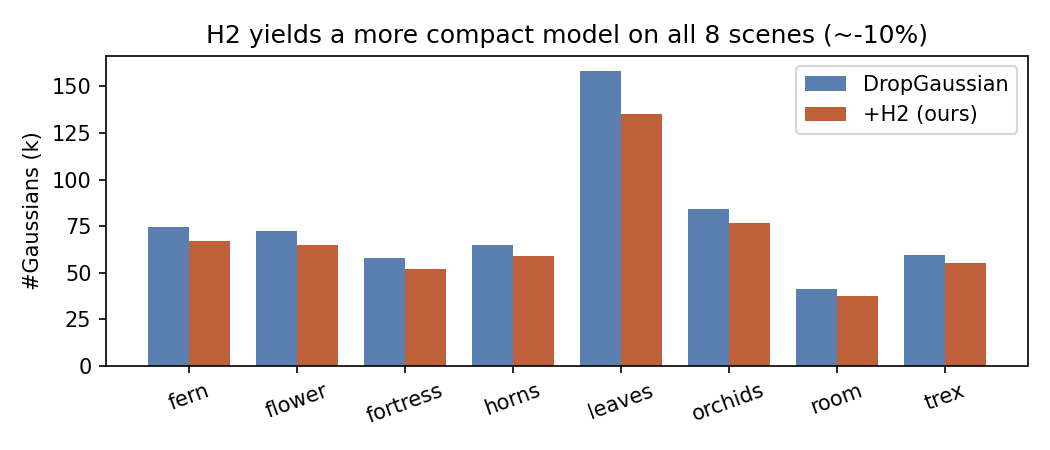
\includegraphics[width=\linewidth]{../results/figs/gauss_bar.png}
\caption{Final Gaussian count, original vs.\ +H2. H2 produces a more compact model on
all eight scenes ($-10.7\%$ mean), a deterministic, noise-free effect.}
\label{fig:gauss}
\end{figure}

\begin{figure}[t]
\centering
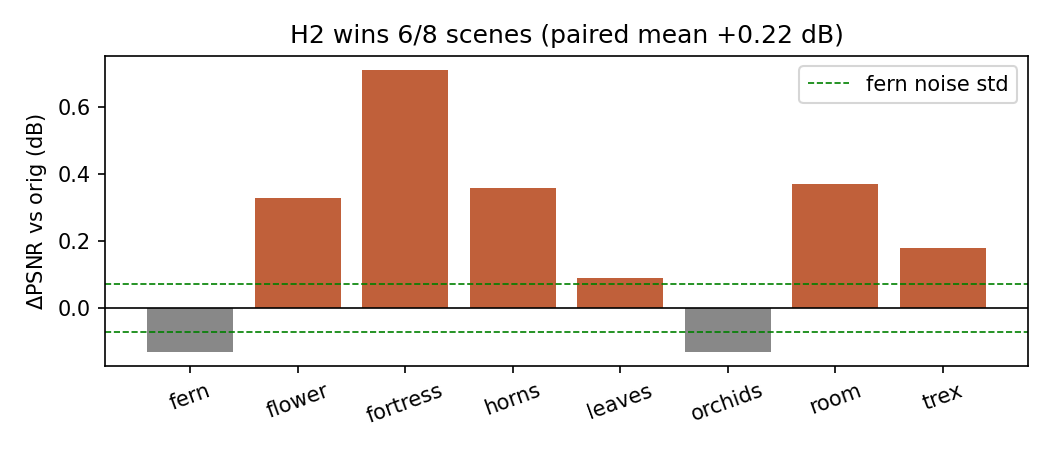
\includegraphics[width=\linewidth]{../results/figs/delta_psnr.png}
\caption{Per-scene $\Delta$PSNR of H2 vs.\ original. Dashed band: $\pm$fern noise std.
H2 wins 6/8; the two small losses lie within the noise band.}
\label{fig:delta}
\end{figure}

\begin{figure}[t]
\centering
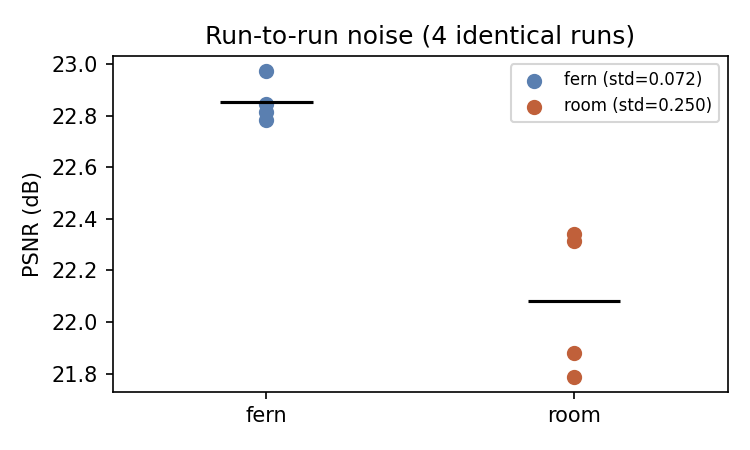
\includegraphics[width=0.85\linewidth]{../results/figs/noise.png}
\caption{Run-to-run PSNR over four identical \emph{original} runs. Non-deterministic
rasterization gives std 0.07\,dB (fern) and 0.25\,dB (room).}
\label{fig:noise}
\end{figure}

\begin{figure}[t]
\centering
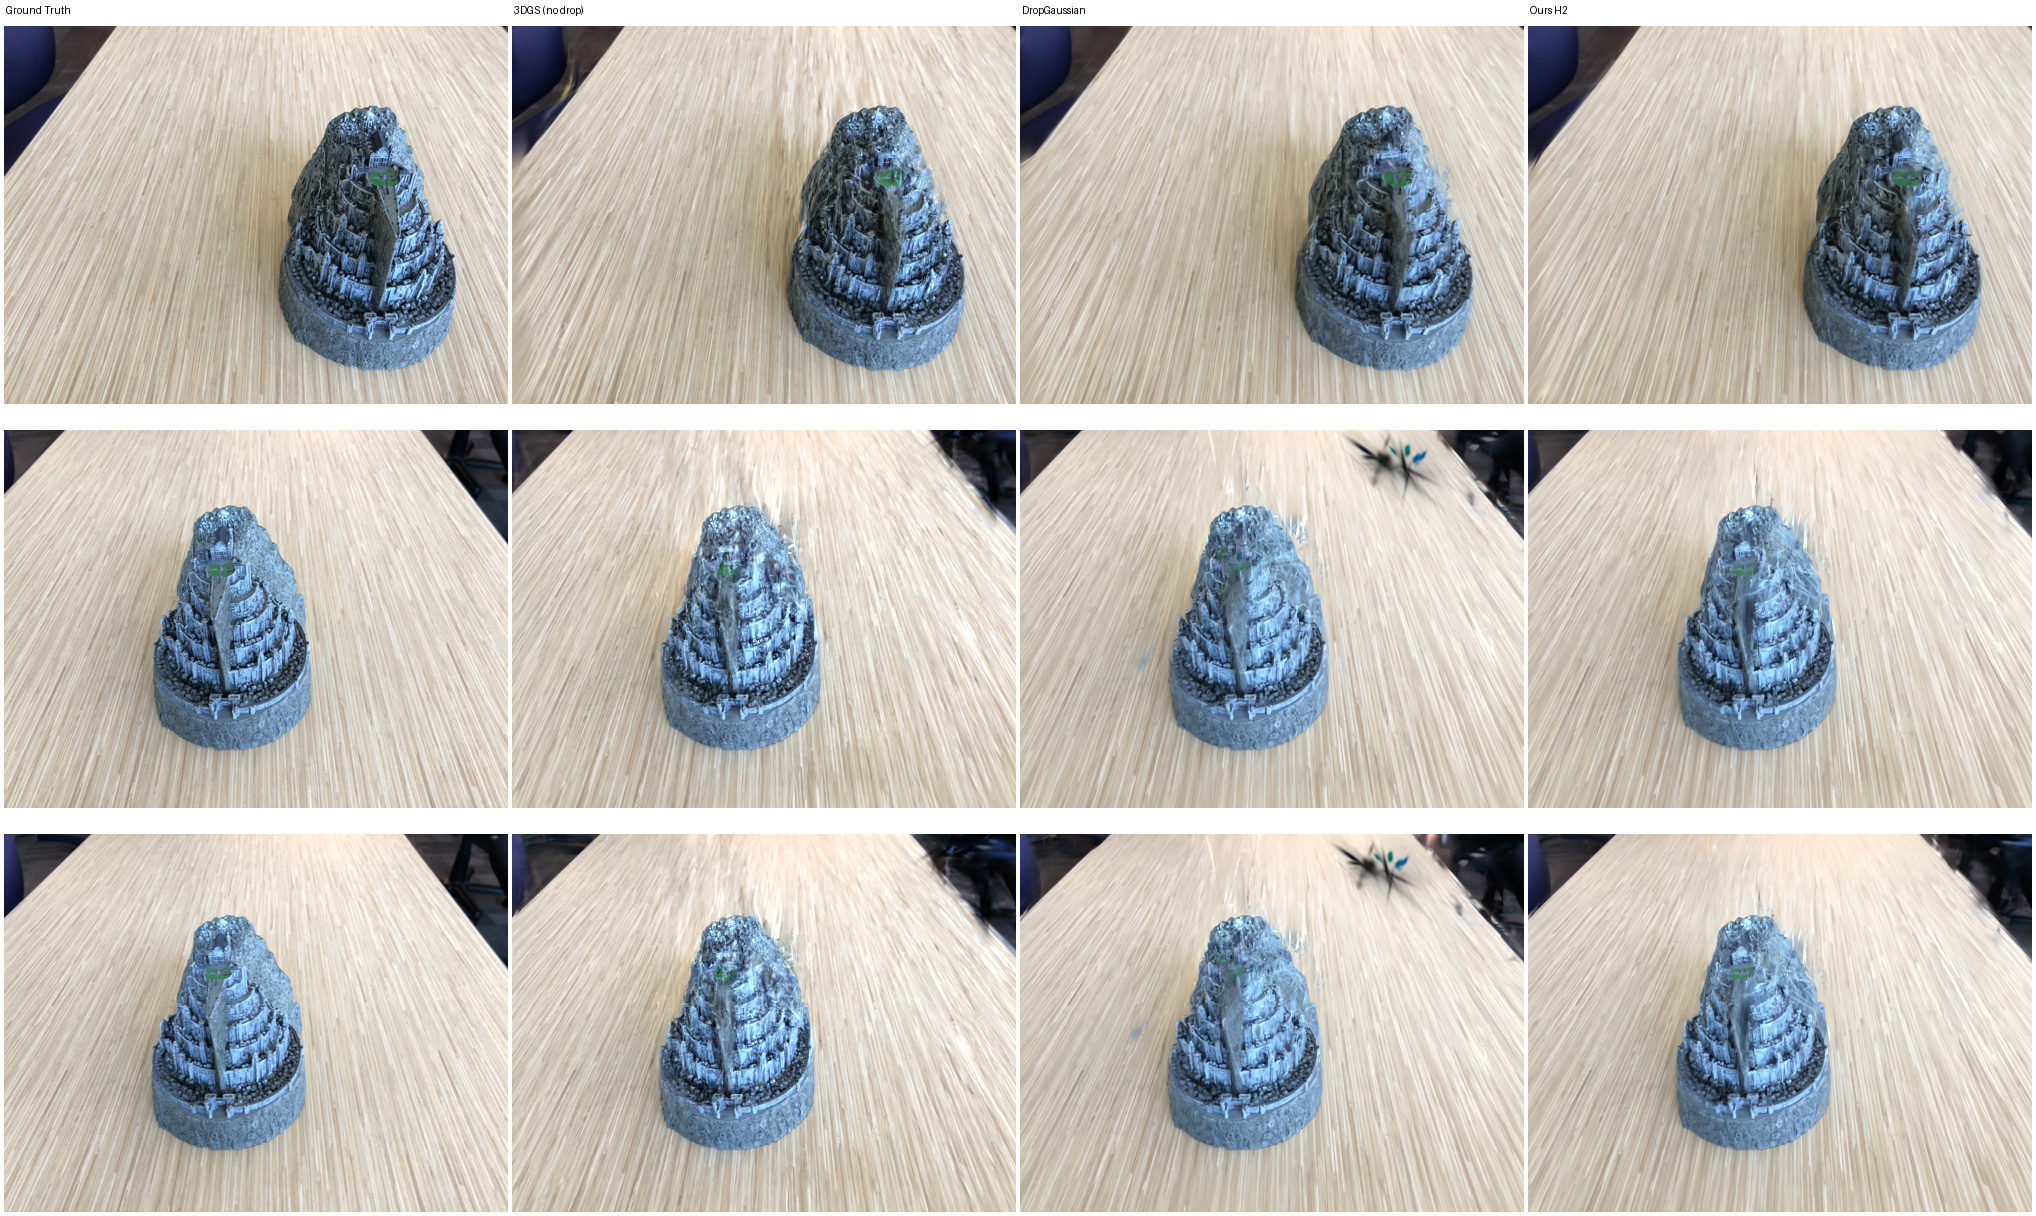
\includegraphics[width=\linewidth]{../results/figs/fortress_compare.png}
\caption{Held-out views (fortress): GT, 3DGS (no drop), DropGaussian, Ours (H2).
Differences are subtle at this PSNR scale, consistent with the quantitative findings;
more scenes (horns, room) are in the data package.}
\label{fig:cmp}
\end{figure}

\textbf{Qualitative (Fig.~\ref{fig:cmp}).} 3DGS shows the most artifacts; DropGaussian
and H2 are visually close, as expected from a sub-dB difference. The improvement is
better characterized quantitatively (compactness) than visually.

\section{Discussion \& Conclusion}
\textbf{Did the hypotheses hold?} \emph{H1: no.} Opacity-aware dropout is $-0.05$\,dB
(wins 3/8) and harms H2 when combined. The reason is mechanistic: DropGaussian works
precisely \emph{because} it occasionally removes dominant high-opacity Gaussians,
forcing the rest to compensate; H1 protects exactly those Gaussians and thereby blunts
the regularizer. The bounded compensation needed to keep variance sane (Sec.~\ref{sec:method})
cannot recover this loss. The hypothesis is cleanly falsified.

\emph{H2: yes, with a nuance.} Drop-aware densification gives $+0.22$\,dB (6/8) and,
more robustly, a deterministic $\sim$10\% reduction in Gaussian count on every scene at
equal-or-better SSIM/LPIPS and no extra cost. The PSNR gain alone sits near the
rasterization noise floor, but the compactness result is noise-free and confirms the L2
mechanism directly. We therefore regard H2 as a genuine, if modest, improvement:
\emph{equal-or-better quality with a leaner, less-overfit model}.

\textbf{Why the gains are small.} DropGaussian is already a strong, carefully-tuned
regularizer. Refining the \emph{shape} of the dropout (H1) or its \emph{coupling} to
densification (H2) operates at the margin and is easily masked by stochastic
rasterization noise. This is an honest near-zero/small result; we deliberately avoid
cherry-picking a single favorable scene, which the noise analysis shows would be
misleading.

\textbf{Limitations \& future work.} Our study is confined to LLFF 3-view; the noise
floor would ideally be estimated per configuration with more repeats. More importantly,
the analysis suggests that \emph{larger, structured} interventions are needed to move
the needle: (i) DropBlock-style \emph{spatial} dropout that removes correlated clusters
of Gaussians rather than i.i.d.\ singletons (directly attacking L1's ``routing-around''
failure), and (ii) overfitting-adaptive drop schedules that allocate more
regularization to early densification, when redundant Gaussians are born. H2 also
suggests a broader principle: any regularizer that alters the forward pass should
re-examine its interaction with adaptive density control.

\section*{AI Usage Statement}
AI tools (Claude) were used to assist with Docker environment setup, debugging, the
code implementation of H1/H2, experiment orchestration/scripting, and the
drafting/polishing of this report. All experiments were executed by the author on the
described hardware, and every reported number is a real measurement from those runs.

\begin{thebibliography}{00}
\bibitem{kerbl3Dgaussians} B. Kerbl, G. Kopanas, T. Leimk\"uhler, and G. Drettakis,
``3D Gaussian Splatting for Real-Time Radiance Field Rendering,'' \textit{ACM Trans.
Graphics}, vol.~42, no.~4, 2023.
\bibitem{park2025dropgaussian} H. Park, G. Ryu, and W. Kim, ``DropGaussian: Structural
Regularization for Sparse-view Gaussian Splatting,'' in \textit{Proc. IEEE/CVF CVPR},
2025.
\bibitem{zhu2024fsgs} Z. Zhu, Z. Fan, Y. Jiang, and Z. Wang, ``FSGS: Real-Time Few-Shot
View Synthesis using Gaussian Splatting,'' in \textit{Proc. ECCV}, 2024.
\bibitem{mildenhall2019llff} B. Mildenhall, P. Srinivasan, R. Ortiz-Cayon
\textit{et al.}, ``Local Light Field Fusion: Practical View Synthesis with Prescriptive
Sampling Guidelines,'' \textit{ACM Trans. Graphics}, vol.~38, no.~4, 2019.
\end{thebibliography}

\end{document}
